\subsection{マイページ機能}

\subsubsection{投稿履歴閲覧機能}
事業者会員自身がこれまでに投稿したピン投稿の履歴を一覧で確認できる機能．ホーム画面の「マイページ」を選択すると，アカウント情報と投稿履歴が表示される．タブ内に投稿履歴があり，選択すると自分自身が過去に行った投稿が表示される．

\begin{figure}[H]
        \centering
        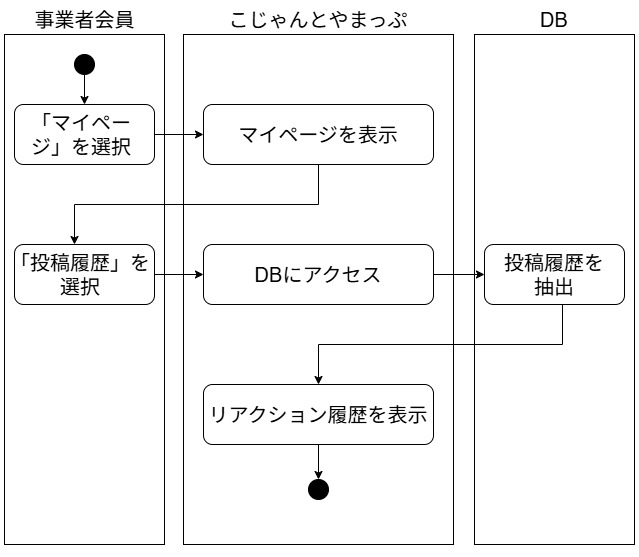
\includegraphics[scale=0.5]{sections/fig_mypage_business/mypage_bus1.jpg}
        \caption{投稿履歴閲覧機能}

        \label{fig:Q17}

\end{figure}

\subsubsection{投稿内容削除機能}
事業者会員自身がこれまでに投稿したものを削除できる機能．ホーム画面の「マイページ」を選択すると，アカウント情報と投稿履歴が表示される．タブ内に投稿履歴があり，選択すると自分自身が過去に行った投稿が表示され，削除したい投稿の右端にあるゴミマークを選択し，「投稿を削除しますか？」に対して「OK」と選択することで投稿が削除される．削除が完了すると「投稿を削除しました」と表示される．

\begin{figure}[H]
        \centering
        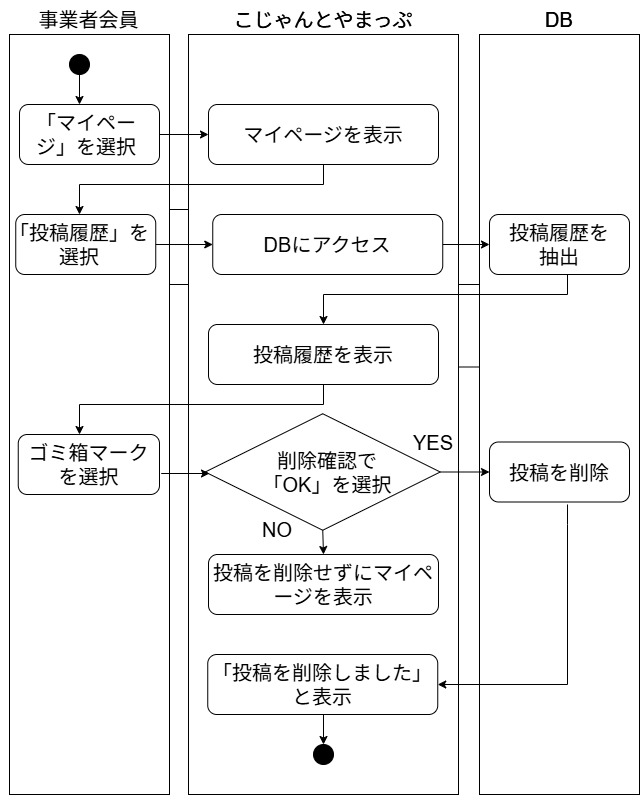
\includegraphics[scale=0.5]{sections/fig_mypage_business/mypage_bus2.jpg}
        \caption{投稿内容削除機能}
        \label{fig:Q18}
\end{figure}

% \subsubsection{ダッシュボード機能}
% 事業者会員自身がこれまでに投稿に対するリアクション数の推移や閲覧数を閲覧できる機能．

% \begin{figure}[H]
%         \centering
%         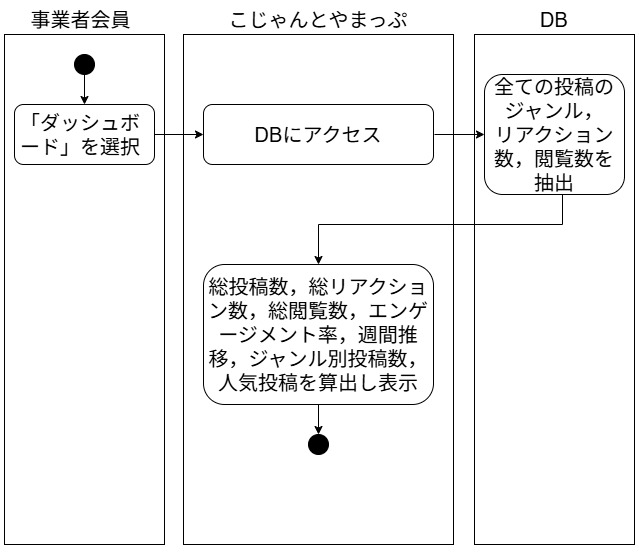
\includegraphics[scale=0.5]{sections/fig_mypage_business/mypage_bus3.jpg}
%         \caption{ダッシュボード機能}
%         \label{fig:Q19}
% \end{figure}

% \subsubsection{支払い状況確認機能}
% 現在の契約状況や支払い履歴，次回の請求日・支払額が確認できる機能．

% \begin{figure}[H]
%         \centering
%         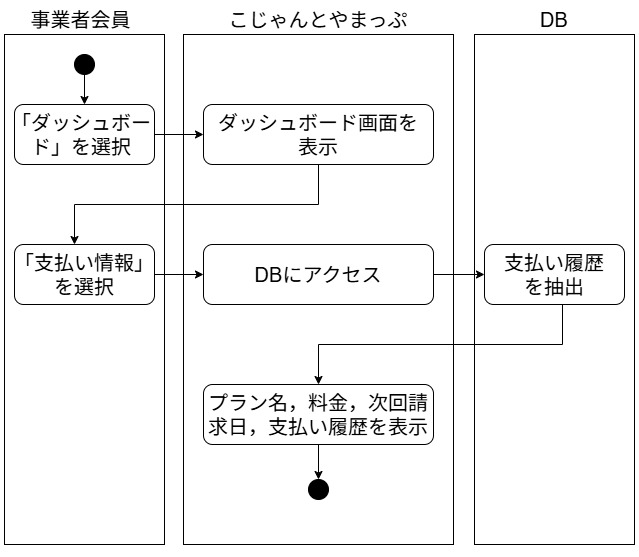
\includegraphics[scale=0.5]{sections/fig_mypage_business/mypage_bus4.jpg}
%         \caption{支払い状況確認機能}
%         \label{fig:20}
% \end{figure}